\chapter{Background}\label{chap:background}
\fancyhead[LO]{\nouppercase{\leftmark}}

\section{Generative deep learning}\label{sec:generative_deep_learning}
In this chapter, I outline the central concepts and objects that form the basis for my method. First, I define (deep) neural networks and state their central property of being general function approximators. Next, I explain the training procedure of neural networks and finish by giving a brief introduction to generative models as a special class of deep learning algorithms. The following sections are loosely based on \cite[Chapter~6, pp.~164-194 and 200-209; Chapter~20, pp.~651-662]{Goodfellow2016}.

\subsection{Definitions}\label{sec:NN-basics}

\begin{definition}\label{mlp-definition}
	For $n, k_1,\dots, k_{n+1} \in \N$ and distinct continuous functions $g_1,\dots, g_n$, where $g_i: \R^{k_i} \to \R^{k_{i+1}}$ for all $i=1,\dots, n$ 
	a \textbf{feedforward neural network (FNN)} $f$ is the function composition
		\begin{equation}
			\begin{split}\label{FNN-form}
			f: \R^{k_1} &\to \R^{k_{n+1}}, \\
			x &\mapsto (g_n\circ g_{n-1} \circ \dots \circ g_2\circ g_1)(x).
			\end{split}
		\end{equation}  
\end{definition}

The term "neural network" stems from a loose analogy between the mathematical models and a biological model of the way information is processed through a network of brain cells or neurons.
The term "feedforward" refers to the fact that such a neural network maps an input value $x$ through the functions that define $f$ to an output value $f(x)$ without allowing for any feedback connections or recurrence. 

A function $g_i: \R^{k_i}\to \R^{k_{i+1}}, i\in \lbrace 1, \dots, n\rbrace$ of the composition $f$ is called a \textbf{layer} of the neural network. Additionally, the input vector $x\in \R^{k_1}$ is often represented as its own layer, called the \textbf{input layer} of the neural network. The last layer, where the transformation $g_n$ is applied to produce the final output $f(x)$ of the neural network, is called \textbf{output layer}, i.e., a neural network satisfying Defitinion~\ref{mlp-definition} always consists of at least one input and one output layer. For $n>1$, the layers between the input and output layer are called \textbf{hidden layers}, and if there is more than one hidden layer, i.e., if $n>2$, the neural network is called \textbf{deep}.

Typically, a $g_i: \R^{k_i}\to \R^{k_{i+1}}, i\in \lbrace 1, \dots, n\rbrace$ is represented as an affine linear transformation followed by a typically non-linear \textbf{activation function}: For some $x\in\R^{k_i}$, $g_i$ would be of the form 
\begin{equation}\label{layer-shape_fnn}
g_i(x) = \phi_i.(W_i x + b_i),
\end{equation}
for a continuous function $\phi_i: \R \to \R$, a matrix $W_i \in \R^{k_{i+1}\times k_i}$ and a vector $b_i \in \R^{k_{i+1}}$, where $\phi.$ denotes the element-wise application of the function $\phi$ to each component of the vector $W_i x + b_i$.

In the following, I assume that each function $g_i: \R^{k_i}\to \R^{k_{i+1}}, i\in \lbrace 1, \dots, n\rbrace$ defining an FNN as in (\ref{FNN-form})  is of the form (\ref{layer-shape_fnn}). The matrices $W_i, i\in \lbrace 1,\dots, n\rbrace$ are called \textbf{weights} of $f$ and the vectors $b_i, i\in \lbrace 1,\dots, n\rbrace$ are called \textbf{biases} of the FNN $f$. The set $\lbrace W_1,\dots, W_n, b_1, \dots, b_n\rbrace$ of all weights and biases is also called the set of \textbf{parameters} of the FNN.

Commonly used activation functions include 

the \textbf{logistic} function $S: \R \to \R, x \mapsto \frac{\exp(x)}{\exp(x)+1}$, 

the \textbf{hyperbolic tangent} function $\tanh: \R\to \R, x\mapsto \frac{\exp(2x) - 1}{\exp(2x) + 1}$ 

and the \textbf{rectified linear unit (ReLU)} function $\mathrm{ReLU}: \R \to \R, x\mapsto \max\lbrace 0,x\rbrace$.

From Definition~\ref{mlp-definition} we see that a neural network is a function composed of a finite number of linear and non-linear transformations. They are also referred to as \textbf{multilayer perceptrons} and form the basic building blocks of deep learning models. 
 
Due to the structure of a feedforward flow of information through a composition of functions not involving recurrence, the mathematical FNNs can be represented as directed acyclic graphs: 
For a layer $i \in \lbrace 1,\dots, n\rbrace$, let $o_i := (g_{i-1} \circ \dots\circ g_1)(x) \in \R^{k_i}$ be the output of the previous layer $i-1$. Typically, the individual dimensions of the output of the current layer $g_i(o_i)^{(1)}, \dots, g_i(o_i)^{(k_{i+1})}$ correspond to the nodes of the graph in layer $i$, that are also called \textbf{units}. The edges of the graph denote the mutual dependencies of the layers as defined by the function compositions.

\begin{figure}
	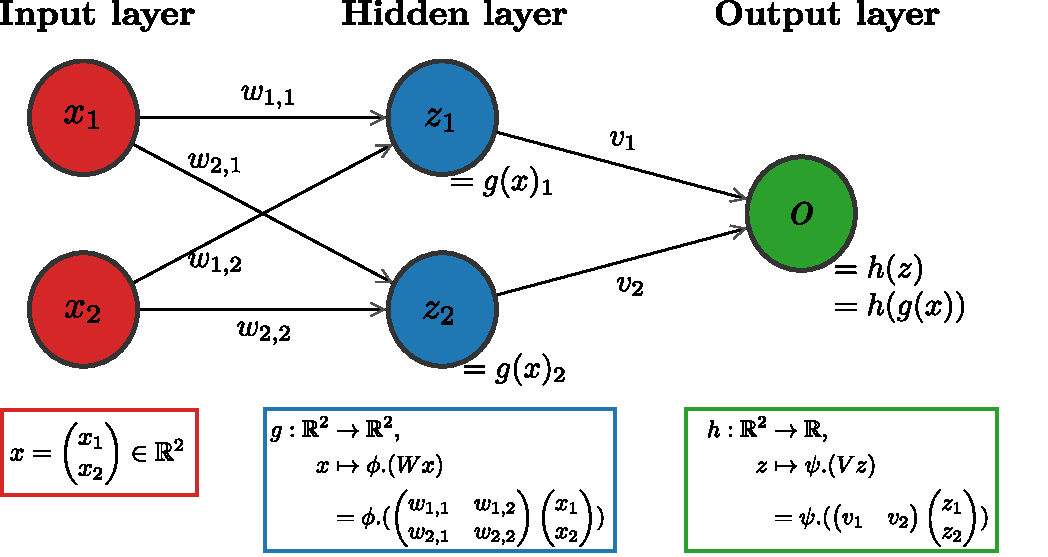
\includegraphics[width=\linewidth]{simple_fnn_example.pdf}
	\caption{Simple FNN example.}
	\label{fig:simple_fnn}
\end{figure}

Figure~\ref{fig:simple_fnn} illustrates the representation of a simple FNN as a directed acyclic graph. Here, the network consists of three layers, an input layer with two nodes, one hidden layer with two nodes and an output layer with one node. The network thus defines a function 
\begin{equation*}
\begin{split}
	f:\R^2 &\to \R, \\
	x&\mapsto f(x) = h(g(x)),
	\end{split}
\end{equation*}
where the functions $g: \R^2 \to \R^2, x \mapsto g(x) = \phi.(Wx)$, $h: \R^2 \to \R, z\mapsto h(z) = \psi.(Vz)$ defining the hidden and output layer, respectively, each consist of a linear transformation with a weight matrix $W\in\R^{2\times 2}$ resp. $V\in\R^2$ followed by a non-linear activation function $\phi:\R\to\R$ resp. $\psi:\R\to\R$. 

\subsection{Neural networks as universal function approximators}\label{sec:nns_universal_approximators}

Generally, FNNs are applied to approximate functions, that, e.g., map some input data $x$ to a label $y$ and thus serve as a classifier. Prior to their successful application in many areas such as pattern and sequence recognition, medical diagnosis, finance or game playing (\cite[pp.~22-26]{Goodfellow2016}), the basic theoretical property of feedforward neural networks as universal function approximators has been investigated and proved in several versions. 

The \textbf{universal approximation theorem} states that a feed-forward neural network with a single layer in addition to the input layer containing a finite number of nodes can approximate any Borel measurable function on a compact subset of a finite-dimensional $\R$-vector space under certain assumptions on the activation function (\cite[pp.~194f.]{Goodfellow2016}). Simple FNNs can thus in theory represent a wide variety of interesting functions when given appropriate parameters; however, the theorem does not say anything about whether those parameters can be actually found by an explicit algorithm. 

One of the first versions of the theorem was formulated and proved by George Cybenko in 1989 (\cite{Cybenko1989} and is presented following \cite[pp.~305-307]{Cybenko1989}.

\begin{definition}
	A function $\sigma: \R \to \R$ is called \textbf{sigmoidal}, if 
	\begin{equation*}
		\sigma(x) \to \begin{cases}
		1 & \text{as} \quad x\to +\infty \\
		0 & \text{as} \quad x\to -\infty.
		\end{cases}
	\end{equation*}
\end{definition}

\begin{theorem}[Universal approximation theorem]\label{universal_approx_thm}
	Let $\sigma$ be a continuous sigmoidal function, let $I_n = [0,1]^n \subset \R^n$ 
	denote the $n$-dimensional unit cube in $\R^n$. Then, functions $G: I_n \to \R$ consisting of finite sums of the form 
	\begin{equation}\label{form-of-G}
	\begin{split}
 		G(x) = \sum_{i=1}^{N} v_i \sigma(w_i^{\top}x + b_i),
	\end{split}
 	\end{equation}
	where $x\in I_n, v_i, b_i \in \R, w_i \in \R^n$ for all $i=1,\dots, N$ are dense in $\mathcal{C}(I_n)$ with respect to the supremum norm, i.e., for any continuous function $f\in \mathcal{C}(I_n)$ and any $\varepsilon >0$, there exist constants $v_i, b_i \in \R$ and vectors $w_i \in \R^n$ for all $i=1,\dots, N$, such that for $G(x)$ as in (\ref{form-of-G})
	\begin{equation*}
	\begin{split}
		\mid G(x) - f(x) \mid < \varepsilon \quad \text{for all } x\in I_n. 
	\end{split}
	\end{equation*}
\end{theorem}

The proof is given for a slightly different scenario of a \textbf{discriminatory} function $\sigma$ and is based on an application of the Hahn-Banach theorem and the Riesz representation theorem. The fact that the Hahn-Banach theorem essentially follows from the axiom of choice already hints at the nature of the universal approximation theorem as a theoretical result without a constructive proof that does not provide us with any practical instruction of how to actually construct these approximating networks for a given function. 

To prove the theorem, we first need to define discriminatory functions: 
\begin{definition}
	A function $\sigma: \R \to \R$ is called \textbf{discriminatory}, if for a measure $\mu$ on $I_n$, it follows from
	$$
	\int_{I_n} \sigma(v^{\top}x + b) d\mu(x) = 0 \quad \text{ for all } v\in\R^n, b \in \R
	$$
	that $\mu \equiv 0$.
\end{definition}

With that definition, we can reformulate the universal approximation theorem as follows:

\begin{theorem}\label{UAT-reformulated}
	Let $\sigma$ be a continuous discriminatory function. Then, finite sums of the form
	\begin{equation}\label{form-of-G-2}
	\begin{split}
		G(x) = \sum_{i=1}^{N} v_i \sigma(w_i^{\top}x + b_i), 
	\end{split}
	\end{equation}
	where $x\in I_n, v_i, b_i \in \R, w_i \in \R^n$ for all $i=1,\dots, N$ are dense in $\mathcal{C}(I_n)$ with respect to the supremum norm. 
\end{theorem}
\begin{proof}
	The following proof is a slightly more detailed version of the proof in \cite[p.~306]{Cybenko1989}.
	Let $\mathcal{G} \subset \mathcal{C}(I_n)$ be the set of functions of the form $G(x)$ as in (\ref{form-of-G-2}). It is clear that $\mathcal{G}$ is a linear subspace of $\mathcal{C}(I_n)$. We prove by contradiction that the closure of $\mathcal{G}$ with respect to the supremum norm is all of $\mathcal{C}(I_n)$. 
	
	Assume for contradiction that the closure $\bar{\mathcal{G}}$ is a proper subspace of $\mathcal{C}(I_n)$. The space $\mathcal{C}(I_n)$ is complete with respect to the supremum norm. Then, it follows from the Hahn-Banach theorem that there is a bounded linear functional $L$ on $\mathcal{C}(I_n)$ with the property that $L\neq 0$ but $L$ vanishes on $\bar{\mathcal{G}}$ and thus also on $\mathcal{G}$. 
	
	$\mathcal{C}(I_n)$ is a Hilbert space with respect to the $L^2$ inner product. Thus, by the Riesz representation theorem, there is a function $l\in \mathcal{C}(I_n)$ such that 
	$$
	L(f) = \langle l,f\rangle_{L^2} = \int_{I_n} f(x)l(x) d\lambda(x) 
	$$ 
	for all functions $f\in\mathcal{C}(I_n)$, where $\lambda$ denotes the Lebesgue measure. 
	
	Then, the function 
	$$
	\mu: \mathcal{B}(I_n) \to \R, \mu(A) := \int_A l(x) d\lambda(x)
	$$
	defines a measure $\mu$ on $I_n$ and $L$ can be written as 
	\begin{equation}\label{form-of-L}
			L(f) = \int_{I_n} f(x) d\mu(x)		
	\end{equation}
	for all $f\in\mathcal{C}(I_n)$. In particular, since obviously $\sigma(v^{\top}(\cdot) + b) \in \bar{\mathcal{G}}$ for all $v \in \R^n, b\in \R$, it follows that
	$$
	L(\sigma(v^{\top}(\cdot) + b)) = \int_{I_n} \sigma(v^{\top}x + b) d\mu(x) = 0
	$$
	for all $v \in \R^n$ and $b\in \R$.
	Since $\sigma$ was assumed to be discriminatory, it follows that $\mu\equiv 0$. We can see from (\ref{form-of-L}) that this implies $L = 0$ on all $\mathcal{C}(I_n)$, contradicting our assumption. Hence, the subspace $\mathcal{G}$ must be dense in $\mathcal{C}(I_n)$.
\end{proof}

The universal approximation theorem, Theorem~\ref{universal_approx_thm}, now follows from Theorem~\ref{UAT-reformulated} and the following lemma: 

\begin{lemma}
	Any bounded, measurable sigmoidal function is discriminatory. In particular, any continuous sigmoidal function is discriminatory.
\end{lemma}
\begin{proof}
	The (rather technical) proof can be found in \cite[pp.~307f.]{Cybenko1989}. 
\end{proof}

It was later shown by Leshno et al. (\cite{Leshno1993}) that FNNs satisfying the assumptions of the universal approximation theorem (Theorem~\ref{universal_approx_thm}) are a universal approximator if and only if the activation function is not polynomial.

In order for FNNs with a single hidden layer to be universal approximators, their layer width can be exponentially large with respect to the desired accuracy. In 2017, Lu et al. (\cite{Lu2017}) proved a universal approximation theorem for deep FNNs with bounded width. In particular, they showed that any Lebesgue integrable function on an $n$-dimensional input space can be approximated with respect to $\mathrm{L}^1$ distance by an FNN of width $n+4$ with ReLU activation functions, if the network depth is allowed to grow.

\subsection{Training neural networks with backpropagation}\label{sec:backprop}
The process of finding a parameter set, i.e., determining weights and biases such that a FNN approximates a specific input-output-mapping is called \textbf{learning} or \textbf{training} of the FNN. The term \textbf{deep learning} thus refers to the process of approximating certain input-output-mappings with deep neural networks. 

More precisely, this is realised by specifying an objective in terms of a \textbf{cost function} that, for example, often denotes a measure of distance between each output value of the FNN and the corresponding training target. If a FNN and the objective are designed such that the cost function is differentiable with respect to the network parameters, we can optimise it by taking its gradient with respect to the parameters and set it to zero, thus "learning" parameters that best approximate the desired mapping, as quantified by the defined objective. 

In this light, nearly all deep learning algorithms can be described as examples of a standard procedure from classical statistical learning: 
Given a dataset, we define a model, a cost function and an optimisation procedure, and aim to optimise the model parameters with respect to the objective specified via the cost function.

If a model includes nonlinearities, such as non-linear activation functions of FNNs, most standard cost functions can no longer be optimised in closed form (\cite[Chapter 5, p.~151]{Goodfellow2016}). This requires an iterative numerical optimisation procedure, such as the gradient descent algorithm, to approximately minimise the cost function. 
Specifically, FNNs are typically trained with the \textbf{backpropagation} algorithm, first developed in \cite{Rumelhart1986} and described by the original authors as follows: "The procedure repeatedly adjusts the weights of the connections in the network so as to minimize a measure of the difference between the actual output vector of the net and the desired output vector." (\cite[p.~533]{Rumelhart1986})
Backpropagation is employed to learn parameters of a neural network such that an arbitrary cost function of the FNN output that is differentiable with respect to the parameters is minimised. 

In the forward pass of one iteration, an input value is passed through all the layers one by one, by applying the function defining the layer with the current set of parameters. 
Having applied all layer functions, the loss for the obtained output value can be calculated.
If we are interested in learning a classifier, i.e., a mapping assigning labels to each input, we also regard the loss as a function of the true label to compare the output to.
Since the output has been derived from applying the FNN function to the input and that function depends on the current parameter values, we can also for a fixed input regard the loss as a function of the network parameters. Assuming it is differentiable with respect to the parameters, we can calculate the partial derivatives of the loss function with respect to each parameter and set the derivatives to zero. 
Due to the structure of the FNN as a function composition, the chain rule has to be applied multiple times to obtain the gradients: The loss directly depends on the parameters of the last layer, which depend on those of the second last layer, etc. In that way, the gradients are propagated backwards through the network to obtain the partial derivative with respect to each parameter -- hence the term backpropagation. After obtaining the partial derivatives with respect to all the parameters, the current parameter values can be updated according to the gradient descent algorithm. Proceeding in this way, the cost function is iteratively optimised with respect to the network parameters and the network is thereby trained to ultimately approximate the desired input-output mapping. Neccessary conditions for this procedure are a scalar loss value for each input and a differentiable FNN structure.

\begin{figure}
	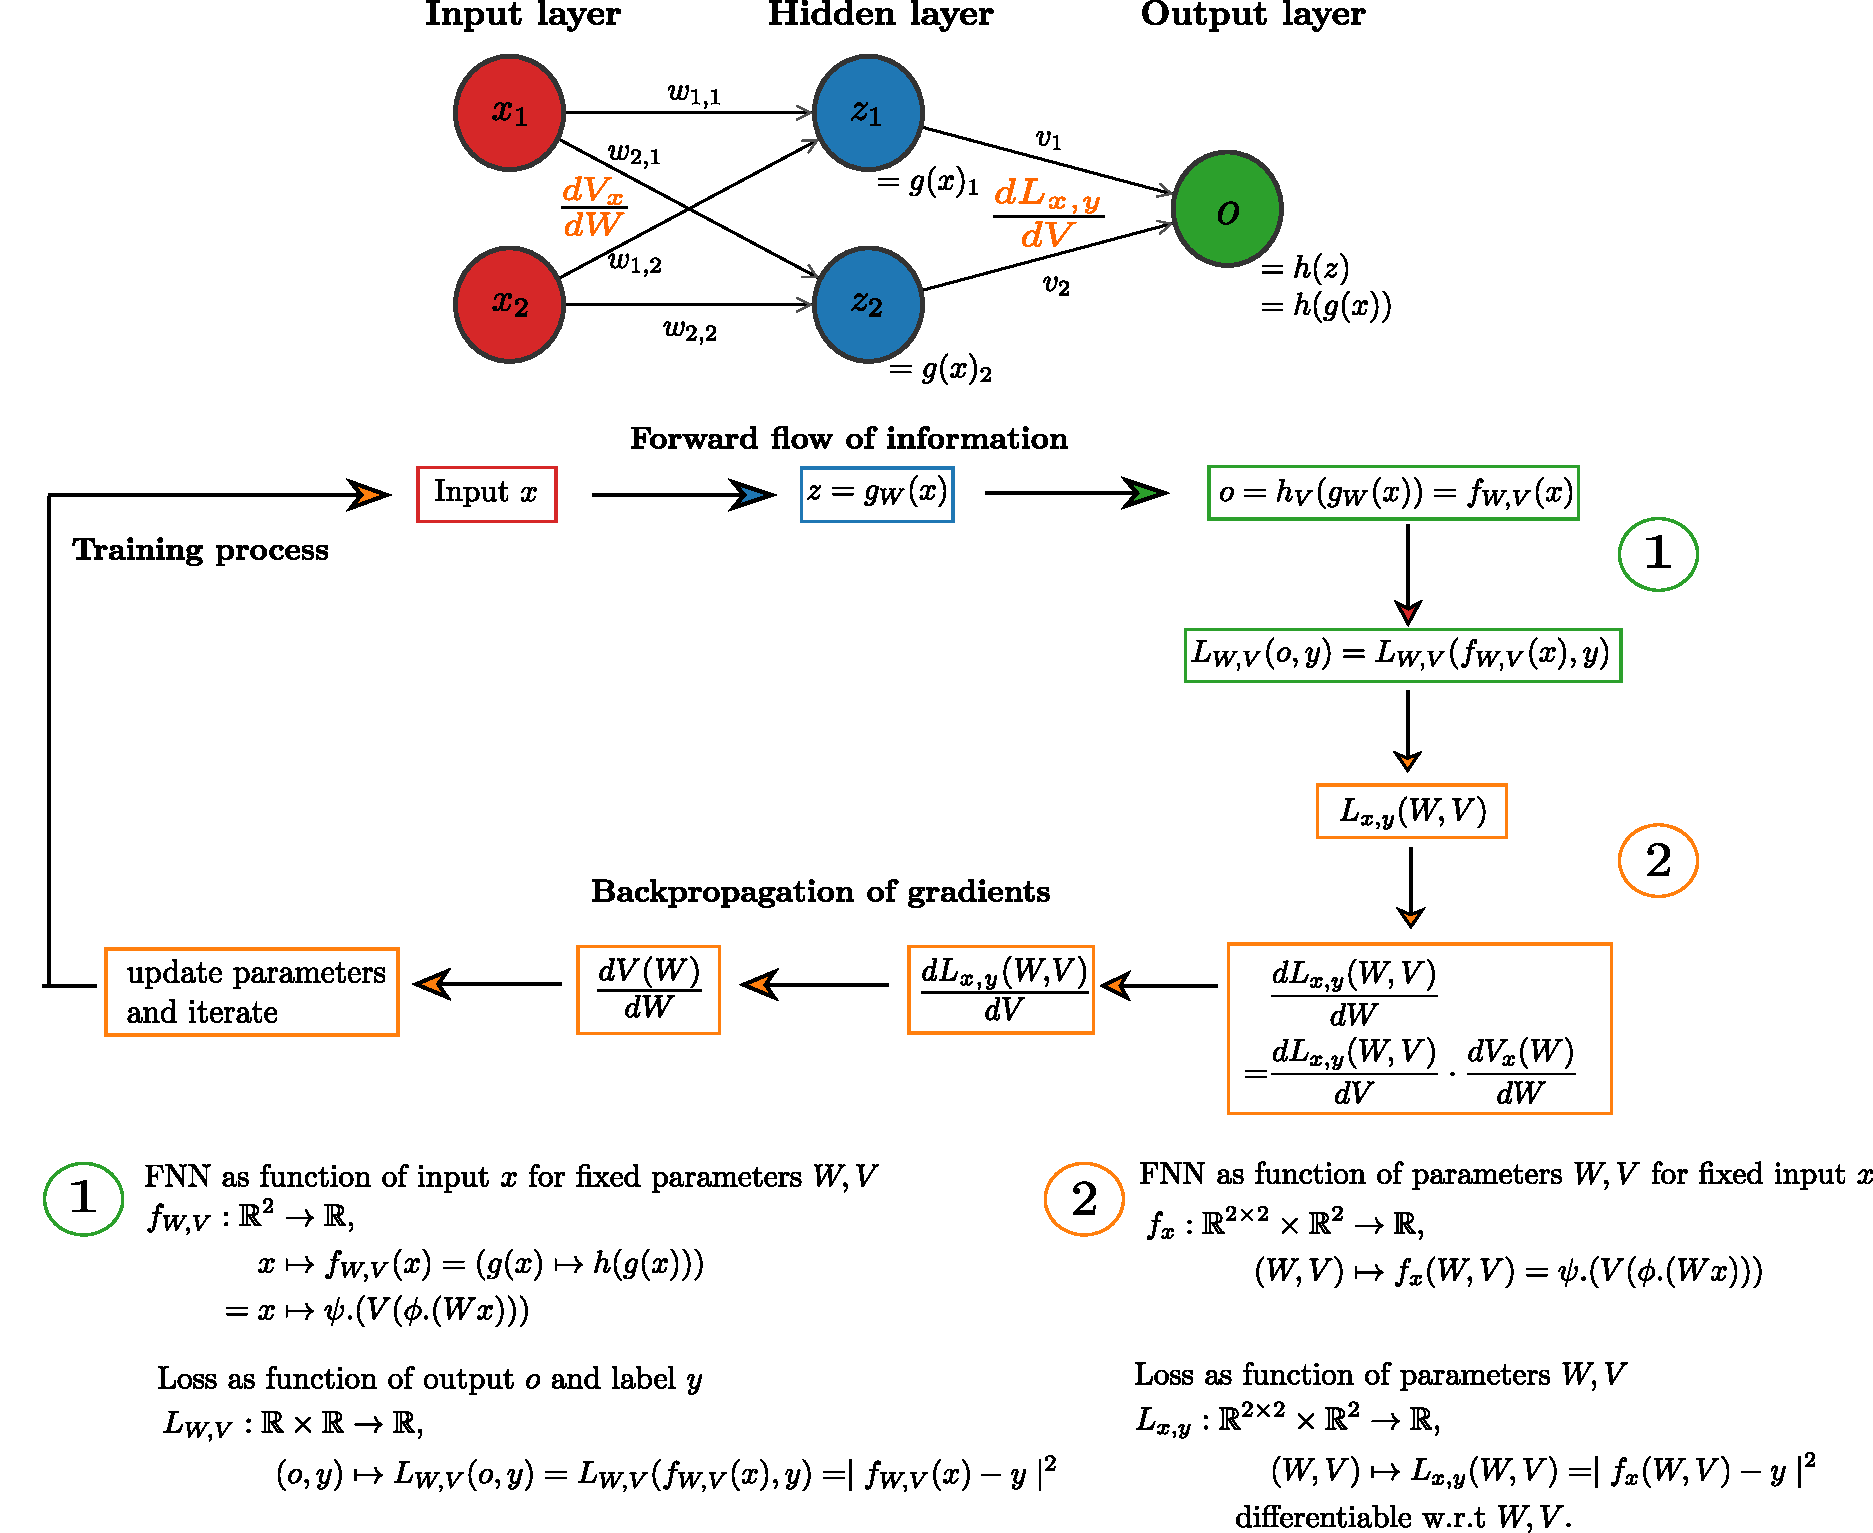
\includegraphics[width=1.1\linewidth]{simple_fnn_backprop.pdf}
	\caption{Training an FNN with backpropagation.}
	\label{fig:backprop}
\end{figure}

Figure~\ref{fig:backprop} illustrates the backpropagation algorithm with the simple FNN example from Figure~\ref{fig:simple_fnn}. The loss function is chosen to be the squared difference between an FNN output and the corresponding true label.

Often the \textbf{stochastic gradient descent (SGD)} algorithm is employed for training, which uses randomly drawn minibatches of data $\mathcal{M} \subset \mathcal{D}$ to obtain an unbiased estimate $\hat{L}(\theta, \varepsilon)$ of the objective $L(\theta)$, i.e., $\E_{\P^{\mathcal{E}}}[\hat{L}(\theta, \cdot)] = L(\theta)$ for FNN parameters $\theta$, where the random variable $\mathcal{E}$ describes the sampling of the minibatch (\cite[p.~72]{Kingma2019}). In the $k$-th step of the SGD algorithm, the current parameter value $\theta_k$ is updated to $\theta_{k+1}$ according to
$$
	\theta_{k+1} \leftarrow \theta_k + \alpha_k \cdot \nabla_{\theta} \hat{L}(\theta, \varepsilon_k),
$$
where $\alpha_k$ denotes the stepsize and is also called the \textbf{learning rate} and $\varepsilon_k$ represents a realisation of $\mathcal{E}$ corresponding to the sampling of the current minibatch. 
Training a FNN can now be achieved by repeating this updating step which is also called a training \textbf{epoch} until a pre-defined convergence criterion of the loss function is reached. 
From now on, all FNNs are assumed to be differentiable with respect to the parameters, thus allowing for an iterative optimisation using (stochastic) gradient descent.

\subsection{Generative models}\label{sec:generative_model_examples}

Neural networks can be trained to approximate different types of input-output relations and have been successfully applied in various classification tasks.
Having learned a classifier and thus being able to discriminate and label new observations does not, however, yield any insight into the data-generating process itself. Additionally, this form of supervised learning typically requires large amounts of labelled training data. After training, the deterministic function represented by such a discriminative neural network will always produce the exact same label for a specific observation and thus does not provide any information about uncertainty on the label assignment (\cite[pp.~2f.]{Kingma2019}). 

To understand the data-generating mechanisms and characterise their variability as a result of random forces governing the process, a \textbf{generative} deep learning model (as opposed to a discriminative one) aims at modelling a joint probability distribution over all the variables (\cite[Chapter~20, p.~651]{Goodfellow2016}). It thus simulates how the data is generated in the real world and accounts for the stochastic nature of that process. A further advantage is that a generative deep learning model can directly learn from data in an unsupervised manner and does not require labelled training examples. 

Having successfully trained a generative model in the form of a neural network then means having captured the process underlying these original observations and formulated it as a probability distribution. As a direct consequence, the model can generate new samples that exhibit the central patterns and structure of the original data. This artificial data can be useful for, e.g., sample size calculations for the planning of future experiments or for settings where due to data protection rules to guarantee privacy it is not possible to share individual-level data.   

While all generative deep learning models share the characteristic of representing a multivariate probability distribution, they differ in the way that distribution is specified. 
In the following, three commonly used examples of deep generative models are briefly reviewed. 

\textbf{Restricted} and \textbf{deep Boltzmann machines (RBMs/DBMs)} are energy-based models, i.e., they define the joint probability distribution of a multi-dimensional binary random vector using an energy function. Originally, they were introduced as a general approach to learning arbitrary probability distributions over binary vectors (\cite{Salakhutdinov09}). The probability distribution is parameterised by a neural network with one (in RBMs) or more (in DBMs) hidden layers. To approximate it, a partition function has to be learned that is generally computationally intractable. However, the specific structure of the neural network allows for efficient Markov Chain Monte Carlo (MCMC) approximation of the desired distributions by using Gibbs Sampling (\cite[Chapter~20, pp.~651-662]{Goodfellow2016}).

Training \textbf{generative adversarial networks (GANs)} (\cite{Goodfellow2014}) can be described as a two-player minimax game of a generator and a discriminator that are both specified by neural networks: Given a dataset and a pre-defined distribution of an input noise random variable, the generative network represents a mapping from the initial distribution to the data distribution the GAN aims to model. The discriminator, a second neural network, outputs the probability that a given input came from the true data distribution rather than from the output distribution of the generator. The discriminator is then trained to maximise the probability of correctly distinguishing between samples from the two, while the generator is simultaneously trained to increase the error rate of the discriminator's classification, i.e., to fool the discriminator. 
The probability distribution function of the original data is thus only available implictly through the samples produced by the generative network.

Finally, a \textbf{variational autoencoder (VAE)}(\cite{Kingma2013}) aims at learning a low-\\
dimensional representation of the input data given by a latent random variable. The transformations from the original data space to the latent space and back are given by independently parameterised, but jointly optimised neural networks: The encoder learns a transformation from the input data to the typically lower-dimensional latent space. It outputs the parameters of an approximation to the posterior distribution of the latent variable given the input data. The generative network is trained to learn the conditional distribution of the input data given a sample of the posterior distribution of the latent variables from the encoder network, such that it approximates the true underlying data distribution. Thus, the encoder is the approximate inverse of the generative model and the two networks are trained jointly, such that the encoder learns a meaningful representation of the input data that can in turn be successfully decoded to samples from the data distribution by the generative network. 

In comparison to GANs, VAEs are reported to have complimentary properties (\cite[p.~5]{Kingma2019}): While GANS can generate subjectively realistic samples, they often only cover a part of the true data distribution, whereas VAEs tend to generate "blurrier", more dispersed samples, but better capture the underlying density. 

Further advantages of the VAE are that it explicitly parameterises the probability distributions involved and that it learns to compress the data into a low-dimensional representation that reflects the central factors of variation governing the dataset. These properties allow us to integrate smoothness constraints and explicit modelling of temporal dynamics into the model and learn a more structured, interpretable low-dimensional representation that provides insight into the main underlying trends driving the temporal patterns in the original data. For these reasons, my own model is based on the framework of a variational autoencoder. In the following sections,I outline the theoretical foundation on which the VAE is build and explain the model architecture and training procedure in detail.  

\section{Variational inference}\label{sec:VI}

\subsection{Prerequisites and notation}\label{sec:inference_basics_notation}
The mathematical framework for the following sections is as follows: 
Let $\Omega := \R^p$, $\mathcal{F} := \mathcal{B}(\R^p)$ and $(\Omega, \mathcal{F}, (\P_{\theta})_{\theta\in \Theta})$ be a parametric statistical model with parameter space $\Theta\subset \R^d$ for some $d\in \N$. Let $\P$ be a probability measure on $(\Omega, \mathcal{F})$, let $X$ be a real-valued $p$-dimensional random variable on $(\Omega, \mathcal{F}, \P)$ with probability distribution $\P^X$, let $\mathcal{D} = \lbrace x_1, \dots, x_n \rbrace $ be a dataset of $n$ independent samples of $X$. We assume that the true distribution $\P^X$ is unknown and attempt to approximate it with a member of the family $(\P_{\theta})_{\theta\in\Theta}$.
Let $Z$ be a second lower-dimensional real-valued variable on $(\Omega, \mathcal{F}, \P)$ with probability distribution $\P^Z$ which we do not observe but assume to govern the underlying mechanism according to which observations of $X$ are generated (see Section~\ref{sec:bayesian_inference}). We assume our parametric family to be flexible enough to include or approximate the true distributions of $X$ and $Z$ and their joint distribution.

Additionally, we assume that for every $\theta \in \Theta$, $\P_{\theta}$ is absolutely continuous with respect to the Lebesgue measure $\lambda$. Then, it follows from the Radon-Nikodym theorem that for every $\theta \in \Theta$, $\P_{\theta}$ admits a density with respect to $\lambda$ that we denote by $p_{\theta} = \frac{dP_{\theta}}{d\lambda}$. We assume the Lebesgue measure to be an equivalent measure for all probability measures $\P_{\theta}$, $\theta\in \Theta$, implying that all densities with respect to the Lebesgue measure are strictly positive. 

In general, I denote random variables with capital letters and their realisations with small letters. To denote densities of random variables (provided they exist), I use small letters with the random variable as a subscript, i.e., $p_Z(\cdot)$ is the density of $Z$. For ease of notation, I abbreviate conditional distributions and densities by writing, e.g., $p_{X\mid z}(x)$ for $p_{X\mid Z=z}(x)$. I write $\E_p[q]$ for the integral $\int_{-\infty}^{\infty}q(x)\cdot p(x)~dx$, where $q$ and $p$ are densities with respect to the Lebesgue measure $\lambda$, such that $\E_p[q] = \E[q(X)]$ for a random variable $X$ on $(\Omega, \mathcal{F}, \P)$ with $\frac{d\P^X}{d\lambda} = p$, and therefore $\E[q(X)] = \int_{\Omega} q(X)~d\P = \int_{-\infty}^{\infty} q(x)\cdot p(x)~dx$.

I denote with $p_X(x,\theta)$ the likelihood function that parameterises the family of potential densities of $X$ as a function of the parameter $\theta$, i.e., evaluates the likelihood of a particular realisation $x$ of $X$ under the density defined by a specific $\theta$. Analoguously, I denote with $p_{X,Z}: \R^2 \times \Theta, (x,z,\theta) \mapsto p_{X,Z}(x,z,\theta)$ for realisations $x$ and $z$ of $X$ and $Z$, respectively, the function parameterising the potential joint densities of $X$ and $Z$ as a function of $\theta$ and also use this notation to parameterise families of potential densities of a single random variable or of conditional probability distributions. For simplicity, I refer to these potential "candidate" densities of distributions or random variables simply as densities.

\subsection{Bayesian inference}\label{sec:bayesian_inference}

The data are assumed to be generated in a two-step process (\cite[p.~2]{Kingma2013}): First, a sample $z$ of a the lower-dimensional random variable $Z$ on $(\Omega, \mathcal{F},\P)$ is drawn according to its distribution $z \sim \P^Z$, called the \textbf{prior distribution}. We assume that $\P^Z = \P_{\theta^{Z}}$ for a $\theta^{Z} \in \Theta$. Secondly, a sample $x = x_{i}$ for some $i\in \lbrace 1,\dots, n\rbrace$ is drawn from the conditional distribution $\P_{X\mid z}$. We assume the joint distribution $\P^{X,Z}$ to also be a member of the family $(\P_{\theta})_{\theta\in\Theta}$, such that the density of the conditional distribution of $(X\vert z)$ for a realisation $z$ of $Z$, given by the expression
$$
p_{X\mid z}(x) :=  \frac{p_{X,Z}(x,z)}{p_{Z}(z)},
$$
can also be parameterised by $\Theta$. We assume that the parameters $\theta^Z$ and $\theta^{(X,Z)}$ characterising the true distribution of $Z$ and the true joint distribution of $X$ and $Z$ are unknown. 

Intuitively, this scenario implies that the variation in our data is based on a few unobserved factors of variation corresponding to the dimensions of the latent random variable $Z$ that we would like to recover along with the details of how the data are generated from the low-dimensional representation $Z$. To achieve that, since only $X$ but not $Z$ is observed, we have to reverse the process and use the observations of $X$ to enrich our knowledge of $Z$, i.e., we condition the distribution of $Z$ on the observations of $X$ and compute the density of the \textbf{posterior distribution} of $Z$ in Bayesian terminology (see \cite[pp.~57-63]{Czado2011}, \cite[p.~70]{Kingma2019} for more on Bayesian inference). According to Bayes' rule, we obtain
\begin{equation}\label{bayes_with_z-posterior}
p_{Z\mid x}(z) = \frac{p_{X,Z}(x, z)}{p_{X}(x)} = \frac{p_{X,Z}(x, z)}{\int p_{X,Z}(x, z) dz}.
\end{equation}

In the last expression of (\ref{bayes_with_z-posterior}), the marginal data likelihood is rewritten as an integral of the joint density of $X$ and $Z$ over all values of $Z$. A model that parameterises such a family of potential joint distributions of the observed and latent variables with FNNs is called a \textbf{deep latent variable model (DLVM)} as in \cite[pp.~12f.]{Kingma2019}. 
Training a DLVM that parameterises $p_{X,Z}$ as a function of $\theta$ means to find the parameters $\theta_{X,Z}$ such that $p_{X,Z}(\cdot, \theta_{X,Z})$ equals the true density of $\P^{X,Z}$.  
In such a DLVM, for a fixed $\theta$ the marginal likelihood of a sample $x$ of $X$ is given by
\begin{equation}\label{marginal-likelihood}
	p_X(x,\theta) = \int_{-\infty}^{\infty} p_{X,Z}(x,z,\theta)dz,	
\end{equation}
which shows that an advantage of these models is their expressivity while maintaining a simple structure: even for relatively simple factors $p_{X,Z}(x,z,\theta)$, the marginal density $p_{X}$ can be very complex and DLVMs can thus effectively model complicated underlying distributions $\P^X$(\cite[pp.~12f.]{Kingma2019}). 

To obtain a maximum likelihood estimate for $\theta$ in DLVMs modelling joint distributions of input data and latent variables, the data likelihood $p_{X}(x,\theta)$ has to be maximised with respect to $\theta$. 
From (\ref{marginal-likelihood}), we see that calculating this marginal likelihood from the joint distribution involves integrating over all possible configurations $(x,z)$. Even for moderately complex models, such as DLVMs with a non-linear hidden layer, this is computationally intractable, implying the intractability of the posterior (\cite[p.~13]{Kingma2019}).

If, however, the density of the conditional distribution $p_{Z\mid x}(\cdot,\theta)$ is tractable to compute, the \textbf{expectation maximisation (EM)} algorithm (\cite{Rubin1977}) can be used to approximate the maximum likelihood estimate of the marginal likelihood, which consists of iteratively applying the following two steps until convergence:

1. \textbf{Expectation step:} Define $q(\theta\mid \theta^{(k)})$ as the expected value of the log likelihood function of the joint distribution of $X$ and $Z$ with respect to the conditional distribution of $Z$ given a sample $x$ of $X$ under the current estimate of $\theta^{(k)}$:
$$
	q(\theta\mid \theta^{(k)}) := \E_{p_{Z\mid x}(\cdot, \theta^{(k)})}\left[\log\left(p_{X,Z}(x, \cdot, \theta)\right)\right].
$$

2. \textbf{Maximisation step:} Find the parameter $\theta^{(k+1)}$ that maximises this quantity:
$$
	\theta^{(k+1)} := \arg \max_{\theta} q\left(\theta\mid \theta^{(k)}\right).
$$

\subsection{Inference as an optimisation problem}\label{sec:inference_as_optimisation}

In DLVMs, the marginal likelihood $p_{X}$ of the data-generating random variable $X$ is typically intractable. But since they are defined as a model parameterising the joint density $p_{X,Z}(x,z,\theta)$, this joint distribution is tractable to compute in DLVMS. Hence, we can see from (\ref{bayes_with_z-posterior}) that the posterior $p_{Z\mid x}(z, \theta)$ is tractable if and only if the marginal likelihood is tractable (\cite[p.~14]{Kingma2019}). 

More broadly, this problem applies to any sufficiently complex Bayesian model including latent variables, since inference in a Bayesian model always amounts to conditioning on data and computing the posterior. If this is not computationally tractable, approximative inference is required (\cite[p.~2]{Blei}). A classical approach for that is Markov chain Monte Carlo (MCMC) sampling, which amounts to constructing a Markov chain on $Z$ such that its stationary distribution is that of the posterior $\P_{\theta}^{Z\mid x}$, sampling from the chain and approximating the posterior with an empirical estimate constructed from the samples (\cite[p.~2]{Blei}). MCMC sampling is a common and widely used tool to perform approximate inference in Bayesian statistics that has been extensively studied (for an overview see, e.g., \cite{Casella2004}). 

\textbf{Variational inference} (\cite{Blei}) represents an alternative strategy to approximate intractable posterior distributions. The key idea is to reframe the problem of performing approximate inference as an optimisation problem rather than using sampling. To this end, we define a family $\mathcal{Q}$ of approximate densities over the latent variables $Z$ and aim to find the member of the family that minimises a measure of distance $d(\cdot,\cdot)$ to the exact posterior density:
\begin{equation}\label{var_inference_generaldistance}
	q^*_{Z\mid x} = \arg \min_{q_{Z\mid x}\in\mathcal{Q}} d(q_{Z\mid x},p_{Z\mid x}).
\end{equation}

Variational inference in general has advantages over MCMC in settings where a faster approximation of a posterior is desired than can be achieved with MCMC algorithms, such as for large datasets or very complex models. For a more detailed discussion of the strength and weaknesses of the two approaches and typical scenarios in which to use either, see \cite[p.~3]{Blei} and the references mentioned there.

\subsection{The Kullback-Leibler divergence}\label{sec:KL-div}

As a measure of distance between probability distributions, the \textbf{Kullback-Leibler (KL) divergence} (\cite[p.~72]{Goodfellow2016}) is used:
\begin{definition}
	Let $(\Omega,\mathcal{F})$ be a measurable space and let $\P$, $\Q$ be probability measures on $(\Omega, \mathcal{F})$ such that $\P$ is absolutely continuous with respect to $\Q$, i.e., admits a density with respect to $\Q$ denoted by $\frac{d\P}{d\Q}$. The \textbf{Kullback-Leibler (KL) divergence} from $\Q$ to $\P$ is defined as
	$$\dkl(\P\Vert \Q) = \int_{\Omega} \log\left(\frac{d\P}{d\Q}\right) d\P.
	$$   
	If $\P$ and $\Q$ are absolutely continuous with respect to the Lebesgue measure $\lambda$, denoting the densities $p=\frac{d\P}{d\lambda}$ and $q=\frac{d\Q}{d\lambda}$, the Kullback-Leibler divergence can be rewritten as an expectation with respect to $P$: 
	$$
	\dkl(\P\Vert \Q) = \E\left[\log\left(\frac{d\P}{d\Q}\right) \right] = \int_{\Omega} \log\left(\frac{d\P}{d\Q}\right) d\P = \int_{-\infty}^{\infty} \log\left(\frac{p}{q}\right) p~d\lambda = \E_{p}\left[\log\left(\frac{p}{q}\right)\right].
	$$
	In this case, I equivalently write $\dkl(p\Vert q)$ for $\dkl(\P\Vert \Q)$.
\end{definition}

\begin{rmk}\label{rmk:kl-div-nonnegative}
	It follows from Jensen's inequality that the Kullback-Leibler divergence is always non-negative:
	\begin{equation*}
	\begin{split}
		\dkl(\P\Vert \Q)  &= \int_{\Omega} \log\left(\frac{d\P}{d\Q}\right) d\P = \int_{\Omega} -\log\left(\frac{d\Q}{d\P}\right) d\P \\
		& \geq -\log \left(\int_{\Omega} \frac{d\Q}{d\P} d\P\right) = -\log \left(\int_{\Omega} d\Q\right) = -\log(1) = 0,
	\end{split}
	\end{equation*}
	where the $\geq$ results from applying Jensen's inequality. 
	
	The KL divergence is equal to $0$ if and only if the two probability measures $\P$ and $\Q$ are equal.
	However, the KL-divergence is not symmetric and hence is not a metric.
	Nonetheless, it is widely used as a notion of distance between two probability distributions in machine learning and statistics. 
\end{rmk}

Quantifying the difference between members of the variational family $\mathcal{Q}$ and the exact posterior with the KL-divergence, our optimisation problem (\ref{var_inference_generaldistance}) becomes
\begin{equation}\label{var_inference_withkl}
	q^*_{Z\mid x} = \arg \min_{q_{Z\mid x}\in\mathcal{Q}} \dkl(q_{Z\mid x}\Vert p_{Z\mid x}).
\end{equation}
The complexity of this optimisation depends on the complexity of the family $\mathcal{Q}$ of candidate approximate densities. While a simpler structure of $\mathcal{Q}$ allows for a simpler and more efficient optimisation, a larger, more flexible family $\mathcal{Q}$ can potentially capture a density closer to the exact posterior. 

\subsection{Calculus of variation}\label{sec:calculus_of_variation}
The term "variational inference" refers to the theory of calculus of variation, a branch of functional analysis, which centers on the fundamental idea of minimising a functional on some (typically infinite-dimensional) function space. A classical example is given by the Dirichlet energy functional
$$
	E: \mathcal{H}^1(U) \to \R, \quad u\mapsto \frac{1}{2}\int_U \Vert \nabla u(x)\Vert^2 dx,
$$
where $U\subset \R^n$ is an open subset and $\mathcal{H}^1(U)$ denotes the Sobolev space on $U$. The functions that minimise the Dirichlet energy and satisfy certain boundary conditions are exactly the solutions of the partial differential equation given by Laplace's equation $-\Delta u(x) = 0$ for all $x\in U$ subject to appropriate boundary conditions.  More generally, many problems in the scope of calculus of variation have applications in the field of partial differential equations. 

In variational inference, the functional to be minimised is given by the distance measure between the probability distributions, often the KL-divergence, while the space of functions over which it is minimised is given by the variational family $\mathcal{Q}$. In my setting, I will exclusively use a parametric family $\mathcal{Q} = (q_{Z}(\cdot,\phi))_{\phi\in\Phi}$ with $\Phi \subset \R^e$ for some $e\in \N$, so that the space of approximate posterior distributions is completely determined by the parameter space $\Phi$ and hence finite-dimensional. Therefore, here the calculus of variation does not have to be employed to solve the approximation problem.

\subsection{The evidence lower bound}\label{sec:ELBO}

The following derivation of the evidence lower bound is based on \cite[pp.~6f.]{Blei} and \cite[pp.~16-18]{Kingma2019}. 

Returning to our optimisation problem of finding $q_{Z\mid x}^*$ as in (\ref{var_inference_withkl}), rearranging the terms of the KL-divergence yields
	\begin{equation}\label{kl-decomposition}
\begin{split}
\dkl(q_{Z\mid x}\Vert p_{Z\mid x})  &= \E_{q_{Z\mid x}}\left[\log\left(\frac{q_{Z\mid x}}{p_{Z\mid x}}\right)\right] \\
&= \E_{q_{Z\mid x}}[\log(q_{Z\mid x})] - \E_{q_{Z\mid x}}[\log(p_{Z\mid x})] \\
&= \E_{q_{Z\mid x}}[\log(q_{Z\mid x})] - \E_{q_{Z\mid x}}\left[\log\left(\frac{p_{X,Z}(x,\cdot)}{p_{X}(x)}\right)\right] \\
&= \E_{q_{Z\mid x}}[\log(q_{Z\mid x})] - \E_{q_{Z\mid x}}[\log(p_{X,Z}(x,\cdot))] + \log(p_{X}(x)),
\end{split}
\end{equation}
where we used the linearity of the expectation and the fact that $\log(p_{X}(x))$ is a constant with respect to $q_{Z\mid x}$. The last line shows that in fact the KL-divergence we aim to minimise depends on $\log(p_{X}(x))$ which we assumed to be intractable. That intractability implies that of the posterior $p_{Z\mid x}$ (as described in Section~\ref{sec:bayesian_inference}) and was our motivation to approximate the posterior with variational inference in the first place. However, the observation that $\log(p_{X}(x))$ is a constant with respect to $q_{Z\mid x}$ also implies that minimising the expression
$\E_{q_{Z\mid x}}[\log(q_{Z\mid x})] - \E_{q_{Z\mid x}}[\log(p_{X,Z}(x,\cdot))]$
is equivalent to minimising $\dkl(q_{Z\mid x}\Vert p_{Z\mid x})$ with respect to $q_{Z\mid x}$, i.e.,
$$
q_{Z\mid x}^* = \arg \min_{q_{Z\mid x}\in\mathcal{Q}} \dkl(q_{Z\mid x}\Vert p_{Z\mid x}) = \arg \min_{q_{Z\mid x}\in\mathcal{Q}} \E_{q_{Z\mid x}}[\log(q_{Z\mid x})] - \E_{q_{Z\mid x}}[\log(p_{X,Z}(x,\cdot))].
$$

Re-organising the terms in the last line of (\ref{kl-decomposition}) and using the non-negativity of the KL-divergence from Remark~\ref{rmk:kl-div-nonnegative}, we obtain
\begin{equation}\label{lowerbound_on_logpx}
\begin{split}
	\log(p_{X}(x)) &= \E_{q_{Z\mid x}}[\log(p_{X,Z}(x, \cdot))] - \E_{q_{Z\mid x}}[\log(q_{Z\mid x})] + \dkl(q_{Z\mid x}\Vert p_{Z\mid x})\\
	&\geq \E_{q_{Z\mid x}}[\log(p_{X,Z}(x, \cdot))] - \E_{q_{Z\mid x}}[\log(q_{Z\mid x})].
\end{split}
\end{equation}
This shows that $\E_{q_{Z\mid x}}[\log(p_{X,Z}(x, \cdot))] - \E_{q_{Z\mid x}}[\log(q_{Z\mid x})]$, the negative of the equivalent objective $\E_{q_{Z\mid x}}[\log(q_{Z\mid x})] - \E_{q_{Z\mid x}}[\log(p_{X,Z}(x, \cdot))]$ defines a lower bound on the marginal data likelihood $\log(p_{X}(x))$. Because the marginal data likelihood is also called the evidence in Bayesian terminology, this expression is called the \textbf{evidence lower bound (ELBO)}
$$
\elbo(x, q_{Z\mid x}) = \E_{q_{Z\mid x}}[\log(p_{X,Z}(x, \cdot))] - \E_{q_{Z\mid x}}[\log(q_{Z\mid x})].
$$
Since minimising the KL divergence with respect to $q$ is equivalent to minimising $\E_{q_{Z\mid x}}[\log(q_{Z\mid x})] - \E_{q_{Z\mid x}}[\log(p_{X,Z}(x, \cdot))]$, which is equivalent to maximising \\
$\E_{q_{Z\mid x}}[\log(p_{X,Z}(x, \cdot))] - \E_{q_{Z\mid x}}[\log(q_{Z\mid x})]$, it follows that minimising the KL-divergence $\dkl(q_{Z\mid x}\Vert p_{Z\mid x})$ is equivalent to maximising the ELBO and 
$$
q_{Z\mid x}^* = \arg \min_{q_{Z\mid x}\in\mathcal{Q}} \dkl(q_{Z\mid x}\Vert p_{Z\mid x}) = \arg \max_{q_{Z\mid x}\in\mathcal{Q}} \elbo(x, q_{Z\mid x}).
$$
From (\ref{lowerbound_on_logpx}) we can see that the KL-divergence $\dkl(q_{Z\mid x}\Vert p_{Z\mid x})$ determines the gap between the ELBO and the marginal data likelihood $\log(p_{X}(x))$ and thus the tightness of the bound. Rewriting the ELBO can give us an intuition about the properties of the optimal variational density (\cite[pp.~6f.]{Blei}):
\begin{equation}\label{elbo_form_recerror_kldivtoprior}
	\begin{split}
		\elbo(x, q_{Z\mid x}) &= \E_{q_{Z\mid x}}[\log(p_{X,Z}(x, \cdot))] - \E_{q_{Z\mid x}}[\log(q_{Z\mid x})] \\
		&= \E_{q_{Z\mid x}}[\log(p_{X\mid Z}(x) p_Z)] - \E_{q_{Z\mid x}}[\log(q_{Z\mid x})] \\
		&= \E_{q_{Z\mid x}}[\log(p_{X\mid Z}(x))] + \E_{q_{Z\mid x}}[\log(p_{Z})] - \E_{q_{Z\mid x}}[\log(q_{Z\mid x})] \\
		&= \E_{q_{Z\mid x}}[\log(p_{X\mid Z}(x))] + \E_{q_{Z\mid x}}\left[\log\left(\frac{p_{Z}}{q_{Z\mid x}}\right)\right] \\
		&= \E_{q_{Z\mid x}}[\log(p_{X\mid Z}(x))] - \dkl(q_{Z\mid x}\Vert p_{Z}).
	\end{split}
\end{equation}
The first term in the last line shows that maximising the ELBO encourages densities placing mass on configurations of latent variables that explain the observed data, while the second term encourages densities that are close to the prior. 

Parameterising the potential candidate prior and posterior densities of $Z$ and $Z\vert x$ for a sample $x\in\mathcal{D}$ with $\theta$ as in Section~\ref{sec:bayesian_inference} and (e.g.) Equation (\ref{bayes_with_z-posterior}), we can define the ELBO as a function of not only the approximate posterior $q_{Z\mid x}$ and the data $x\in\mathcal{D}$, but also of the parameter $\theta$ defining the densities of $Z$ and $Z\vert x$ that is called the \textbf{model parameter}. Additionally, we assume a parametric variational family $\mathcal{Q} = (q_{Z\mid x}(\cdot, \phi))_{\phi \in \Phi}$ with $\Phi \subset \R^e$ for an $e\in \N$, so that the finite-dimensional space $\Phi$ completely characterises the family of approximate posteriors, and call the parameter $\phi \in \Phi$ the \textbf{variational parameter}. 
As a result, we can view the ELBO as a function of the data $x\in \mathcal{D}$, the model parameter $\theta$ and the variational parameter $\phi$ 
\begin{equation}\label{elbo-as-function-of-theta-and-phi}
\begin{split}
	\elbo(x,\theta, \phi) &= \E_{q_{Z\mid x}(\cdot,\phi)}[\log(p_{X,Z}(x, \cdot, \theta))] - \E_{q_{Z\mid x}(\cdot,\phi)}\left[\log\left(q_{Z\mid x}(\cdot, \phi)\right)\right] \\
	&= \E_{q_{Z\mid x}(\cdot,\phi)}[\log(p_{X\mid Z}(x,\theta))] - \dkl(q_{Z\mid x}(\cdot,\phi)\Vert p_{Z}(\cdot,\theta)).
\end{split}
\end{equation}

Note that since the ELBO is a lower bound on $\log(p_{X}(x,\theta))$, maximising the ELBO with respect to $\theta$ yields an approximation to the maximum likelihood estimate for $\theta$. That approximation is better the smaller the KL-divergence 
$$\dkl(q_{Z\mid x}(\cdot,\phi)\Vert p_{Z\mid x}(\cdot,\theta)),$$ 
that determines the tightness of the bound. We can thus obtain both approximate maximum likelihood estimates for $\theta$ and an optimal variational density $q$ if we maximise the ELBO both with respect to $\theta$ and $\phi$. The search of finding optimal parameters $\theta$ is referred to as \textbf{learning} and the process of finding parameters $\phi$ of an optimal approximate posterior $q$ as \textbf{inference} (\cite[p.~15]{Kingma2019}).

\subsection{Variational expectation maximisation}\label{sec:variational_EM}

Maximising the ELBO with respect to both $\theta$ and $\phi$ can be formulated as a variation of the EM-algorithm from Section~\ref{sec:bayesian_inference} called the \textbf{variational expectation maximisation} algorithm and can also be viewed as coordinate ascent on the ELBO (\cite[p.~71]{Kingma2019}, \cite{NealHinton1998}). It assumes a parametric variational familiy $\mathcal{Q} = (q_{\phi}(z))_{\phi\in\Phi}$ with $\Phi \subset \R^e$ for some $e\in \N$ and estimates \textbf{local} variational parameters $\phi_i$ for each individual sample $x_i$.

As for classical EM, the algorithm starts with (random) initial values of $\theta^{(0)}$ and $\phi_{i=1,\dots, n}^{(0)}$ and iteratively applies the following steps: 

1. \textbf{Expectation step:} For all $i=1,\dots, n$, maximise the ELBO with respect to $\phi_i$ and define
\begin{equation}\label{e-step_variationalEM}
\phi_i^{(k+1)} := \arg \max_{\phi} \elbo(x_i,\theta^{(k)}, \phi_i).
\end{equation}

2. \textbf{Maximisation step:} Maximise the ELBO with respect to $\theta$ and define
\begin{equation}
\theta^{(k+1)} := \arg \max_{\theta} \sum_{i=1}^n \elbo(x_i,\theta, \phi_i^{(k+1)}).
\end{equation}

Note that, as shown before, the objective in (\ref{e-step_variationalEM}) is equivalent to finding $\arg \min_{\phi} \dkl(q_{Z\mid x}(\cdot,\phi) \Vert p_{Z\mid x}(\cdot,\theta^{(k)}))$.

\section{Variational autoencoder}\label{sec:VAE}

The variational autoencoder, briefly described in Section~\ref{sec:generative_model_examples}, is a framework to efficiently perform approximate inference and learning. In short, it is a generative deep learning model consisting of two coupled, jointly optimised neural networks that parameterise an approximate posterior of a latent random variable given observations and the conditional distribution of the data given a sample from the posterior over the latent variables. The training objective is given by the ELBO (\ref{elbo-as-function-of-theta-and-phi}) that is optimised with respect to both the model parameters and the variational parameters using SGD. The following presentation is based on the paper first proposing VAEs \cite{Kingma2013} and \cite[pp.~15-27]{Kingma2019}.

\subsection{Model overview}\label{sec:VAE_model_overview}
The VAE proposes a solution to the three related problems in the setting of intractabilities of the marginal likelihood 
$$p_X(\cdot,\theta) = \int p_{X,Z}(\cdot,z,\theta)dz$$ 
and/or the posterior density
$p_{Z\mid x}(\cdot,\theta)$
for a potentially large dataset where sampling-based MCMC methods would be too slow, namely efficient approximation of maximum likelihood estimates for the parameters $\theta^Z, \theta^{(X,Z)}$, efficient approximate posterior inference of $Z\vert X$ and efficient approximate marginal inference of the underlying variable $X$ (\cite[pp.~2f.]{Kingma2013}). 
Since the latent variable $Z$ encodes a low-dimensional representation of data, the VAE can be seen as a method for inferring these ideally semantically meaningful, statistically independent factors of variation in data. This process is generally known as unsupervised representation learning, and VAEs have been extensively employed for that purpose (\cite[p.~4]{Kingma2019}).

To handle the intractabilities of the marginal likelihood and posterior, a parametric family of distributions $\mathcal{Q}= (q_{Z\mid x}(\cdot, \phi))_{\phi\in\Phi}$ with $\Phi\subset \R^e$ for some $e\in \N$ is introduced. We then aim to optimise the variational parameters $\phi$ to find a family member $q_{Z\mid x}(\cdot, \phi)$ that approximates the true posterior as in Section~\ref{sec:VI}, such that $q_{Z\mid x}(z, \phi) \approx p_{Z\mid x}(z,\theta)$ for all $z\in \R$, $x\in \mathcal{D}$.

The model $q_{Z\mid x}(z, \phi)$ as a function of the variational parameters $\phi$ and realisations $x$ and $z$ of the respective random variables is called the \textbf{inference model} or the \textbf{encoder}, since it encodes a sample $x \in \mathcal{D}$ into a lower-dimensional representation in the space of samples of $Z$. The density $q_{Z\mid x}(\cdot, \phi)$ is parameterised with a deep neural network, i.e., the parameters are given as output of a FNN. 

A second neural network is employed to define the density $p_{X\mid z}(\cdot,\theta)$ called the \textbf{generator} or \textbf{decoder} part of the model. Given an input observation $x$, we obtain a sample $z$ from the distribution given by the density $q_{Z\mid x}(\cdot, \phi)$ that we can use to evaluate the likelihood of the input observation $x$ under the density $p_{X\mid z}(\cdot,\theta)$. Both parts together form the \textbf{variational autoencoder} and can be jointly trained by maximising the ELBO with respect to both the variational parameters $\phi$ and the parameters $\theta$ of our assumed statistical model. 
Note that in contrast to the Variational EM algorithm in Section~\ref{sec:variational_EM}, a single encoder neural network is used that is shared by all observations. Thus, a shared set of variational parameters is estimated, rather than local parameters determined for each individual. This strategy of sharing varational parameters across data points is also called \textbf{amortised variational inference} (\cite[p.~16]{Kingma2019}).

The cost function defining the training objective for the model is given by the negative ELBO (\ref{elbo-as-function-of-theta-and-phi}): Since it is a function of the model parameters $\theta$ and the variational parameters $\phi$ and therefore of the output of two FNNs, maximising it with respect to both $\theta$ and $\phi$ is equivalent to jointly training the encoder and decoder network with backpropagation as described in Section~\ref{sec:backprop}. As noted before, this is equivalent to jointly performing both variational inference by finding optimal parameters of the approximate variational posterior and performing approximate maximum likelihood estimation on the marginal data likelihood by finding optimal model parameters. Note that by applying variational inference to approximate the posterior, the distribution of the latent variable does not have to be specified explicitly beforehand and no specific structure other than dimensionality of the latent representation has to be assumed a priori. Instead, one can simply define a variational family that determines the complexity of the optimisation problem and let the model freely infer a representation that fits the data. 

Having trained the model, we can sample $z$ from the prior and generate an artificial observation $\hat{x}$ by sampling from the distribution defined by $p_{X\mid z}(\cdot,\theta)$.

\subsection{Stochastic gradient-based optimisation of the ELBO}\label{sec:ELBO-optimisation}

Training the VAE model means optimising the ELBO with respect to both the model parameters $\theta$ and the variational parameters $\phi$. To perform stochastic gradient descent, the ELBO has to be differentiated with respect to $\theta$ and $\phi$. 
In the following, we derive unbiased estimators of the individual-datapoint ELBO and its gradients (that are generally intractable) based on \cite[pp.~19-23]{Kingma2019} and \cite[pp.~3-5]{Kingma2013}. 

Obtaining an unbiased estimator of the gradient with respect to the generative model parameters $\theta$ is straightforward. For any $x \in \mathcal{D}$ and a sample $z$ from the posterior $q_{Z\mid x}(\cdot,\phi)$ it holds that
\begin{equation}\label{montecarloest1}
\begin{split}
	\nabla_{\theta} \elbo(x,\theta, \phi) &= \nabla_{\theta} \E_{q_{Z\mid x}(\cdot,\phi)}[\log(p_{X,Z}(x, \cdot, \theta)) - \log(q_{Z\mid x}(\cdot, \phi))] \\
	&= \E_{q_{Z\mid x}(\cdot,\phi)}[\nabla_{\theta}(\log(p_{X,Z}(x, \cdot, \theta)) - \log(q_{Z\mid x}(\cdot, \phi)))],
\end{split}
\end{equation}
and (\ref{montecarloest1}) can be estimated with the Monte Carlo estimator 
$$	\nabla_{\theta}(\log(p_{X,Z}(x, z, \theta)) - \log(q_{Z\mid x}(z, \phi))) = \nabla_{\theta}(\log(p_{X,Z}(x, z, \theta))), \quad z \sim q_{Z\mid x}(\cdot,\phi).
$$
Obtaining an unbiased estimator of the gradient with respect to the variational parameters $\phi$ is more challenging, since we take the expectation with respect to $q_{Z\mid x}(\cdot,\phi)$ which depends on $\phi$, and in general

\begin{equation*}
\begin{split}
	\nabla_{\phi} \elbo(x,\theta, \phi) &= \nabla_{\phi} \E_{q_{Z\mid x}(\cdot,\phi)}[\log(p_{X,Z}(x, \cdot, \theta)) - \log(q_{Z\mid x}(\cdot, \phi))] \\
	&\neq \E_{q_{Z\mid x}(\cdot,\phi)}[\nabla_{\phi}(\log(p_{X,Z}(x, \cdot, \theta)) - \log(q_{Z\mid x}(\cdot, \phi)))].
\end{split}
\end{equation*}

To derive an unbiased estimate of $\nabla_{\phi} \elbo(x, \theta, \phi)$, a change of variables called the \textbf{reparameterisation trick} (\cite[pp.~20f.]{Kingma2019}, \cite[pp.~4f.]{Kingma2013}) can be employed. For that, we define a real-valued random variable $\mathcal{E}$ on $(\Omega, \mathcal{F}, \P)$ that is independent of $X$ and $(Z\vert x)$ and a differentiable, invertable transformation $g$ such that for a given parameter value $\phi$ and a sample $x \in \mathcal{D}$ of $X$, we can express
$$
	(Z\vert x) = g(\mathcal{E}, \phi, x).
$$
With that change of variables from $(Z\vert x)$ to $\mathcal{E}$, the expectation with respect to $q_{Z\mid x}(\cdot, \phi)$ can be rewritten in terms of an expectation with respect to $p_{\mathcal{E}}$, the density of $\P^{\mathcal{E}}$. For $x\in \mathcal{D}$ as before, we thus obtain
\begin{equation}\label{montecarloest2}
\begin{split}
	\nabla_{\phi} \elbo(x, \theta, \phi) &= \nabla_{\phi} \E_{q_{Z\mid x}(\cdot, \phi)}[\log(p_{X,Z}(x, \cdot, \theta)) - \log(q_{Z\mid x}(\cdot, \phi))] \\
	&= \nabla_{\phi} \E_{p_{\mathcal{E}}}[\log(p_{X,Z}(x, g(\cdot, \phi, x), \theta)) - \log(q_{Z\mid x}(\cdot, \phi))] \\
	&= \E_{p_{\mathcal{E}}}[\nabla_{\phi}(\log(p_{X,Z}(x, g(\cdot, \phi, x), \theta)) - \log(q_{Z\mid x}(\cdot, \phi)))].
\end{split}
\end{equation}
Now, (\ref{montecarloest2}) can be estimated as before with the Monte Carlo estimator 
$$
\nabla_{\phi}(\log(p_{X,Z}(x, z, \theta)) - \log(q_{Z\mid x}(z, \phi))), \quad z=g(\varepsilon,\phi,x), \quad \varepsilon \sim p_{\mathcal{E}}.
$$
Furthermore, we can see that this estimator is unbiased:
\begin{equation*}
\begin{split}
	\E_{p_{\mathcal{E}}}[\nabla_{\phi}(&\log(p_{X,Z}(x, g(\cdot, \phi, x), \theta)) - \log(q_{Z\mid x}(g(\cdot, \phi, x), \phi)))] \\
			&= \nabla_{\phi}(\E_{p_{\mathcal{E}}}[\log(p_{X,Z}(x, \cdot, \theta)) - \log(q_{Z\mid x}(g(\cdot, \phi, x), \phi))]) \\
			&= \nabla_{\phi}(\E_{q_{Z\mid x}(\cdot, \phi)}[\log(p_{X,Z}(x, \cdot, \theta)) - \log(q_{Z\mid x}(\cdot, \phi))]) \\
			&= \nabla_{\phi}(\elbo(x,\theta, \phi)).
\end{split}
\end{equation*}

As a result, we obtain unbiased estimates of the ELBO with respect to both $\theta$ and $\phi$ and can optimise is using SGD (see Section~\ref{sec:backprop}). Figure~\ref{fig:reparam_trick} illustrates the reparameterisation trick. Note that in general, the ELBO is a non-convex function and thus potentially has several local optima.  

\begin{figure}
	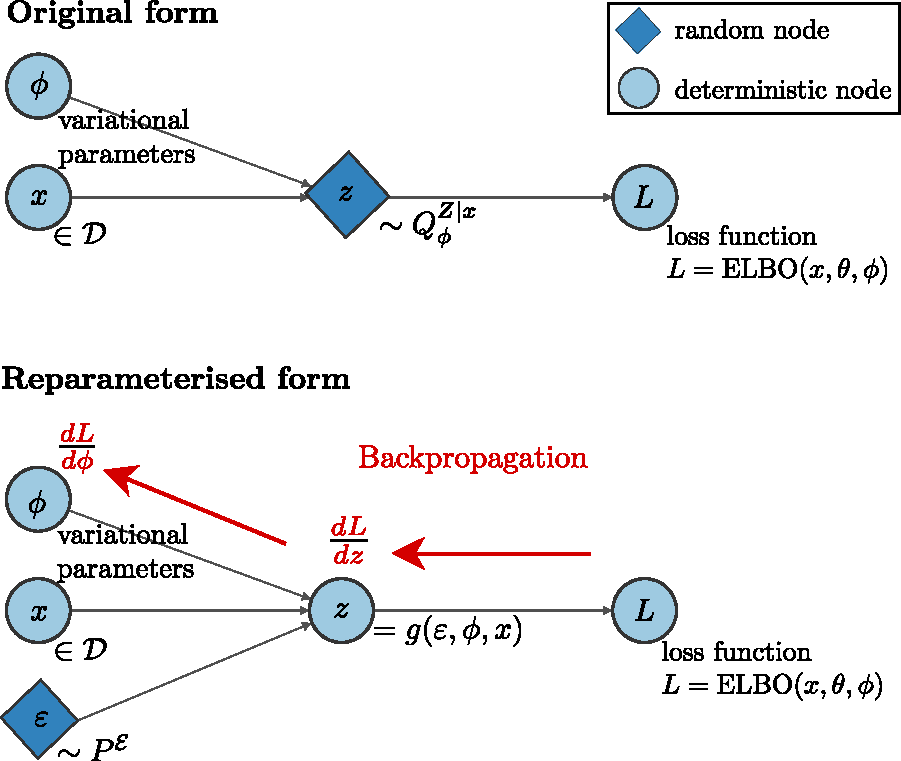
\includegraphics[height=8cm]{reparameterisation_trick.pdf}
	\caption{The reparameterisation trick. (adapted from \cite[p.~22]{Kingma2019})}
	\label{fig:reparam_trick}
\end{figure}

The complete training algorithm of the VAE, also termed \textbf{auto-encoding variational Bayes} algorithm by the original authors (\cite[p.~21]{Kingma2019}, \cite[p.~4]{Kingma2013}), is summarised in Algorithm 1. The training process is visualised in Figure~\ref{fig:VAE_with_reparam}.

\begin{algorithm}
	\SetAlgoLined
	\KwData{ \\Input: dataset $\mathcal{D} = \lbrace x_1,\dots, x_n\rbrace$, \\ 
		Inference model: family of variational posterior distributions $(\Q_{\phi}^{Z\mid x})_{\phi \in \Phi}$, \\
		Generative model: family of joint distributions $(\P_{\theta}^{X,Z})_{\theta\in \Theta}$}
	\KwResult{ \\ Learned parameters $(\theta, \phi)$ of the generative and inference model}
	
	$(\theta, \phi)\leftarrow$ Random initialization\;
	\While{SGD not converged}{
		Sample random minibatch of data $\mathcal{M} \sim \mathcal{D}$\;
		\For{each datapoint $x \in\mathcal{M}$}{
			Sample random noise $\varepsilon \sim \P^{\mathcal{E}}$\;
			Calculate $z = g(\varepsilon, \phi, x)$\;
		}{
		Compute (estimators of) $\elbo(\mathcal{M},\theta, \phi)$ and gradients $\nabla_{\theta, \phi}(\elbo(\mathcal{M},\theta, \phi))$\;
		Update parameters $\theta$ and $\phi$ using SGD optimiser\;
		}
	}
	\caption{Auto-encoding variational Bayes algorithm:	VAE training by stochastic optimisation of the ELBO}
	\label{algo-1}
\end{algorithm}

\begin{figure}
	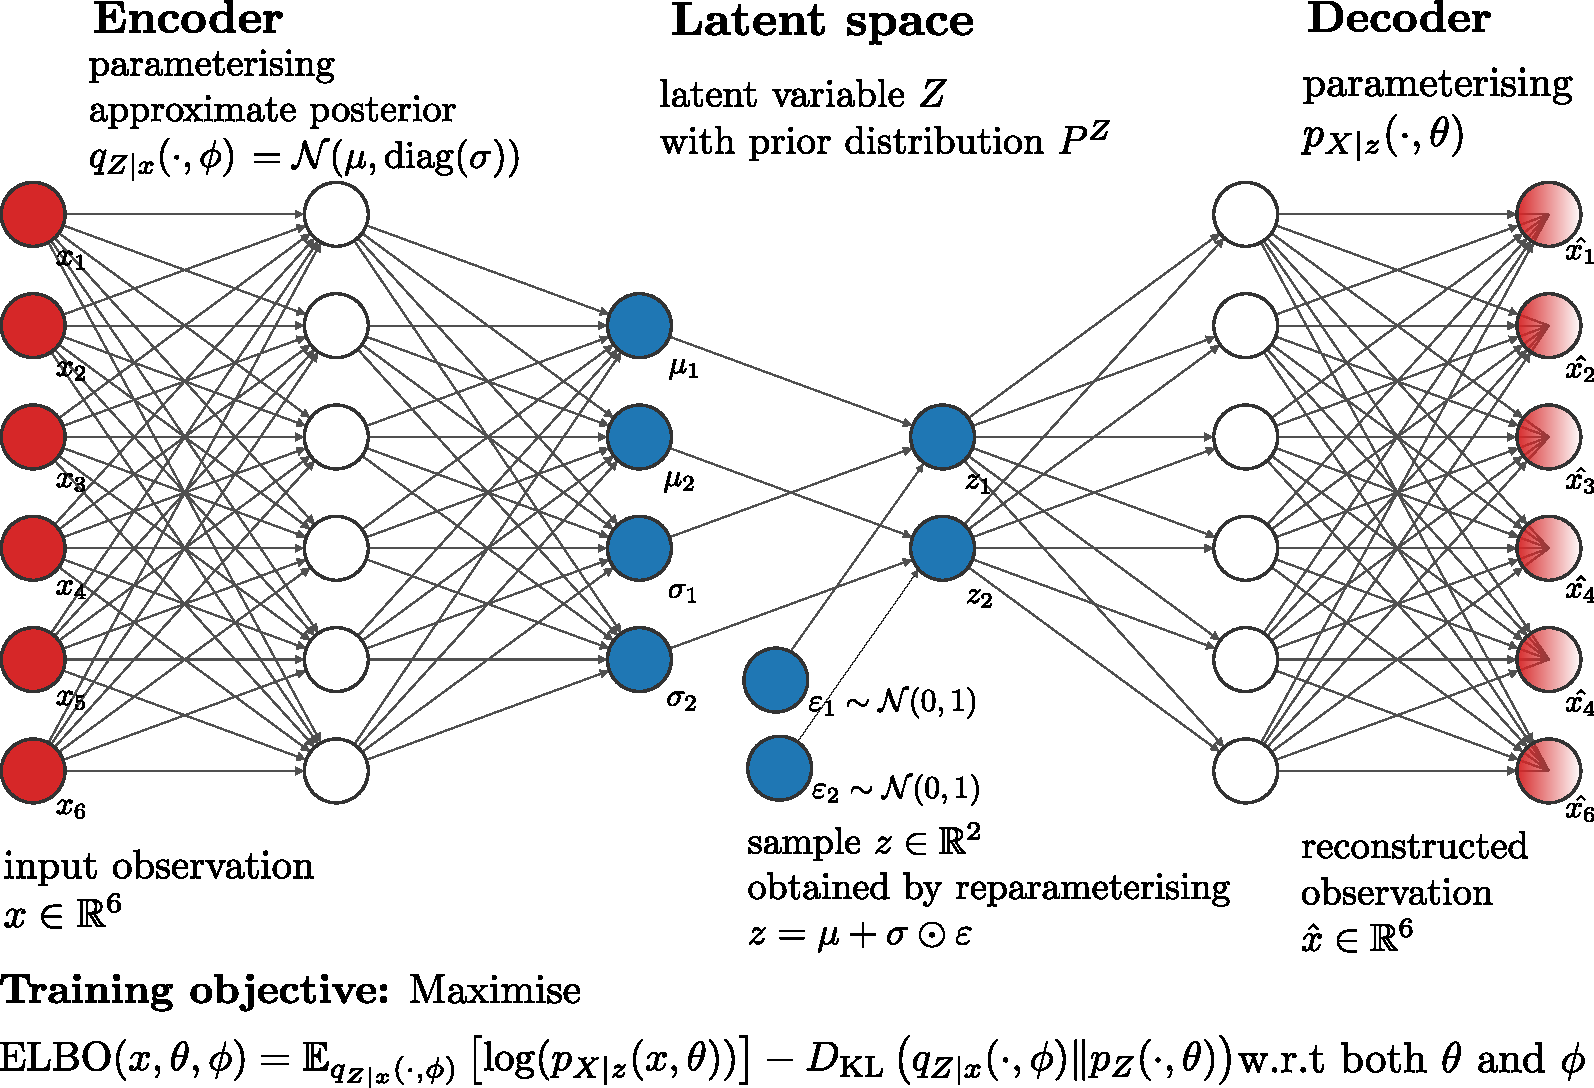
\includegraphics[height=9cm]{vae_with_reparameterisation.pdf}
	\caption{VAE training process with reparameterisation trick.}
	\label{fig:VAE_with_reparam}
\end{figure}

\subsection{Example: VAE with factorised Gaussian posterior}\label{sec:VAE-example_Gaussian_posterior}

In this section, I present a typical and commonly used example of a variational autoencoder with the standard choices for the distributions which enable an efficient computation of the ELBO and thus allow for efficient optimisation (\cite[pp.~24f.]{Kingma2019}, \cite[p.~5]{Kingma2013}). 

Let the prior over the latent variable $Z$ be given by a standard normal distribution, i.e., $Z\sim \P^Z = \mathcal{N}(0,I)$. In this case, the prior has no parameters and is thus not subject to any optimisation or change during training. Let $p_{X\mid z}(\cdot,\theta)$ be the density of a multivariate Gaussian (for real-valued data) or a Bernoulli distribution (for binary data). The distribution parameters $\theta$ are computed from realisations of the latent variable $Z$ with a neural network with a single hidden layer and non-linear activation function. 
In this case, the true posterior $p_{Z\mid x}(\cdot,\theta)$ is intractable. To approximate it, we choose a multivariate Gaussian distribution with mean $\mu \in \R^K$ and diagonal covariance matrix $\mathrm{diag}(\sigma^2)\in \R^{K\times K}$, where the variational parameters $(\mu, \sigma)$ are given by a neural network: 
\begin{equation}
\begin{split}
	(\mu, \log(\sigma)) &= \mathrm{EncoderNeuralNet}(x) \\
	q_{Z\mid x}(z,\phi) &= \prod_{k=1}^K q_{Z\mid x}(z_k,\phi) = \prod_{k=1}^K f_{\mathcal{N}(\mu,\mathrm{diag}(\sigma^2))}(z_k).
\end{split}
\end{equation}
This factorised Gaussian encoder corresponds to the mean-field approach from variational inference, where we also assume the members of the variational family to be mutually independent, such that the distribution factorises (\cite[pp.~7-10]{Blei}).

Choosing $\P^{\mathcal{E}} = \mathcal{N}(0,I)$, we can, for a sample $\varepsilon$ from $\P^{\mathcal{E}}$ and an observation $x$, obtain a sample $z$ from the posterior $\Q_{\phi}^{Z\mid x}$ via the reparameterisation 
$$
	z = \mu + \sigma \odot \varepsilon, 
$$
where $\odot$ denotes the element-wise product. Analogously to the Gaussian example, for any family of distribution defined by a "location" and a "scale", we can choose the standard distribution with location $0$ and scale $1$ for the auxiliary random variable $\mathcal{E}$ and set $z = \mathrm{location} + \mathrm{scale} \odot \varepsilon$. Additionally, also for families of posterior distributions $\left(q_{Z\mid x}(\cdot, \phi)\right)_{\phi\in\Phi}$ with a tractable inverse cumulative distribution function, a differentiable transformation $g$ and an auxiliary variable $\mathcal{E}$ can be chosen such that we can perform the reparameterisation trick (see for details \cite[p.~5]{Kingma2013}).

We have seen in (\ref{elbo_form_recerror_kldivtoprior}) that for any $x \in \mathcal{D}$
$$
	\elbo(x,\theta, \phi) = \E_{q_{Z\mid x}(\cdot, \phi)}[\log(p_{X\mid z}(x,\theta))] - \dkl(q_{Z\mid x}(\cdot, \phi) \Vert p_{Z}(\cdot,\theta)).
$$
The KL-divergence between two multivariate Gaussian distributions with $\mu_1,\mu_2 \in \R^K, \Sigma_1, \Sigma_2 \in \R^{K\times K}$ can be computed in closed form according to the formula
\begin{equation}\label{formula_explicit_KL}
\begin{split}
	\dkl(&\mathcal{N}(\mu_1,\Sigma_1)\Vert \mathcal{N}(\mu_2,\Sigma_2)) \\
	&= \frac{1}{2} \left(\mathrm{tr}(\Sigma_2^{-1}\Sigma_1) 
	+ (\mu_2 - \mu_1)^{\top}\Sigma_2^{-1}(\mu_2 - \mu_1) 
	- K 
	+ \log\left(\frac{\det(\Sigma_2)}{\det(\Sigma_1)}\right)\right).
\end{split}
\end{equation}
We thus obtain for the given choices of the prior and posterior the explicit expression
\begin{equation}
\begin{split}
	\dkl(q_{Z\mid x}(\cdot, \phi) \Vert p_Z)
	&= \dkl(\mathcal{N}(\mu,\mathrm{diag}(\sigma^2))\Vert \mathcal{N}(0,I)) \\
	&= \frac{1}{2}\left(\sum_{k=1}^K \sigma_k^2 + \mu_k^2 - 1 - \log\left(\sigma_k^2\right)\right).
\end{split}
\end{equation}

Using $L$ samples $z^{(1)}, \dots, z^{(L)}$ from the posterior by sampling $\varepsilon^{(1)}, \dots, \varepsilon^{(L)}$ from $\P^{\mathcal{E}} = \mathcal{N}(0,I)$ and calculating $z^{(l)} = \mu + \sigma \odot \varepsilon^{(l)}$, we thus obtain the following estimator for the ELBO at datapoint $x\in \mathcal{D}$:
\begin{equation}
	\elbo(x, \theta, \phi) = \frac{1}{2} \sum_{k=1}^{K}(1+\log(\sigma_k^2) - \mu_k^2 - \sigma_k^2) + \frac{1}{L}\sum_{l=1}^{L} \log(p_{\theta}(x\mid z^{(l)})).
\end{equation}

Here, the decoding term $\log(p_{X\mid z^{(l)}}(x,\theta))$ can be seen as a negative reconstruction error.
A theoretical justification of the particular choice of $q$ is the fact that the Gaussian distribution maximises the entropy, i.e., is the potentially most informative distribution to use if we have no prior knowledge on the structure desired (\cite[pp.~644f.]{Goodfellow2016}).

\section{Ordinary differential equations}\label{sec:ODEs}

Differential equations relate functions and one or more of their derivatives and thus form the paradigmatic concept to describe quantities changing over time. In the following sections, I  formally define differential equations and give basic central results about the existence and uniqueness of solutions. 

\subsection{Definitions}

\begin{definition}[{\cite[p.~27, Definition~1]{Perko2001}}]\label{def:ODE}
	Let $I\subset \R$ be an interval, $U\subset I\times \R^m$ open and $f:U\to\R^n$ a continuous function. Then, for an interval $J\subset I$, a function $x:J\to \R^n$ is called a \textbf{solution of the (ordinary) differential equation} $x' = f(\cdot, x)$ \textbf{on the interval $J$}, if $x$ is differentiable and
	$\frac{d}{dt} x(t) = f(t,x(t))$ for all $t\in J.$

	Additionally, given a $t_0\in J$ and $(t_0,x_0)\in U$, $x$ is called a \textbf{solution of the initial value problem} defined by $f$ and $(t_0,x_0)$ in $J$, if $x$ is a solution of the differential equation and $x(t_0) = x_0$, i.e., if
	\begin{equation*}
	\begin{split}
		\frac{d}{dt} x(t) &= f(t,x), \\
		x(t_0) &= x_0 \text{~for all~} t\in J.
	\end{split}
	\end{equation*} 
	\end{definition}

\begin{rmk}
	Definition~\ref{def:ODE} can be generalised to differential equations of higher orders: For an $n\in\N$, an open subset $U\subset I\times \R^n$ and a continuous function $f$ on $U$, a function $x\in\mathcal{C}^n(J)$ for $J\subset I$ is a solution of the differential equation $x^{(n)}(t) = f(t,x, x', x'',\dots, x^{(n-1)})$ in $J$, if 
	$$
	\tfrac{d^{(n)}}{dt} x(t) = f(t,x(t),\tfrac{d}{dt}x(t), \dots, \tfrac{d^{(n-1)}}{dt}x(t)) \text{~for all~} t\in J.
	$$
	Such a differential equation of order $n$ can always be reduced to a first-order differential equation as in Definition~\ref{def:ODE} by changing to the new set of variables $y = (x, x', x'', \dots, x^{(n-1)})$, which yields the first-order system
	\begin{equation*}
		\begin{split}
			y_1' &= y_2, \\
			&\;\;\vdots \\
			y_{n-1}' &= y_n \\
			y_n' &= f(t,y).
		\end{split}
	\end{equation*}
	Then, any function $x\in\mathcal{C}^n(J)$ is a solution of $x^{(n)}(t) = f(t,x, x', x'',\dots, x^{(n-1)})$ in $J$ if and only if the function $t\mapsto y(t)$ is a solution of the first-order differential equation $y' = f(\cdot, y)$ in $J$ (\cite[p.~7]{Teschl2012}). 
	
	For the corresponding initial value problem, let $(t_0,x_0,\dots, x_{n-1})\in U$ for $t_0\in J$. Then, $x\in\mathcal{C}^n(J)$ is a solution of the initial value problem defined by $f$ and $(t_0,x_0,\dots, x_{n-1})$ in $J$, if $x$ is a solution of the differential equation and additionally $x(t_0) = x_0, \frac{d}{dt}x(t_0) = x_1,\dots, \frac{d^{(n-1)}}{dt} x(t) = x_{n-1}$. 
	We thus see that for an initial value problem of order $n$, in addition to the initial value in $t_0$, the values of the first $n-1$ derivatives in $t_0$ have to be specified. 
\end{rmk}

\begin{rmk}
	Differential equations according to Definition~\ref{def:ODE} are called \textbf{ordinary differential equations (ODEs)}, because the solution function depends on only one variable that is denoted by $t$ in the definition. In contrast to that, equations specifying a relation between partial derivatives of a function of two or more variables or of a vector with two or more dimensions and the function itself are called \textbf{partial differential equations (PDEs)}. An example is the Laplace equation briefly mentioned in Section~\ref{sec:calculus_of_variation} given by 
	$$
	\Delta u(x_1,\dots, x_n) = \sum_{i=1}^{n} \frac{\partial^2}{\partial x_i^2}u(x_1,\dots, x_n) = 0.
	$$
\end{rmk}

\subsection{Existence and uniqueness of solutions}

The main result on the conditions under which initial value problems have solutions is given by the Picard-Lindelöf theorem, which proves local existence and uniqueness for a locally Lipschitz-continuous function $f$ defining the differential equation: 

\begin{theorem}[{Picard-Lindelöf, \cite[p.~38, Theorem~2.2]{Teschl2012}}]\label{thm:picard-lindelöf} Let $U\subset \R\times \R^m$ be an open subset, let $(t_0,x_0)\in U$ and $f:U\to\R^n$ be a continuous function. If $f$ is locally Lipschitz continuous in the second argument, uniformly with respect to the first argument, then there exists a unique local solution of the initial value problem defined by $f$ and $(t_0,x_0)$. More specifically, if $V = [t_0,t_0 + T]\times \overline{B_{\delta}(x_0)} \subset U$ and $M = \max_{(t,x)\in V} \vert f(t,x)\Vert$, the solution exists at least for $t\in [t_0,t_0 + T_0]$ and remains in $\overline{B_{\delta}(x_0)}$, where $T_0 = \min\lbrace T,\frac{\delta}{M}\rbrace$. The analoguous result holds for $[t_0-T,t_0]$.
	\begin{proof}
		I sketch the main steps of the proof and refer to \cite[pp.~36-38]{Teschl2012} for details. 
	 	The central idea is to reframe the statement of the theorem as a fixed-point equation of a functional on a complete metric space. Then, the claim follows from Banach's fixed-point theorem. 
	 	
		First, we observe that a function $x\in\mathcal{C}^1(J,\R^n)$ is a solution of the initial value problem defined by $f$ and $(t_0,x_0)$ in $J$ if and only if the function $x\in\mathcal{C}(J,\R^n)$ solves the integral equation (\cite[p.~36]{Teschl2012})
		$$	x(t) = x_0 + \int_{t_0}^{t} f(s,x(s)) ds.$$ 		
		Note that in order to satisfy the Lipschitz conditions, if suffices that $f\in \mathcal{C}^1(U)$: It then follows from the fact that any continuous function on a compact subset of a finite-dimensional real vector space attains its maximum in that subset (see \cite[p.~71f.]{Perko2001} for details) that for every compact set $V_0\subset U$ the number 
		$$ L = \sup_{(t,x)\neq(t,y)\in V_0} \frac{\vert f(t,x) - f(t,y) \vert}{\vert x-y\vert} $$
		is finite (\cite[p.~37]{Teschl2012}). 
		
		Next, we define the function space 
		$$ \mathcal{X}_I := \lbrace x\in \mathcal{C}(I,\R^n): \sup_{t\in I} \vert x(t) - x_0\vert <\delta\rbrace $$ 
		for some $\delta > 0$ and an interval $I\subset \R$, and a functional $K_I$ on $\mathcal{X}_I$ 
		\begin{equation*}
			\begin{split}
					K_I: \mathcal{X}_I &\to \mathcal{C}(I,\R^n), \\
					(t\mapsto x(t)) &\mapsto \left( t\mapsto T_I(x)(t) := x_0 + \int_{t_0}^{t}f(s,x(s)) ds\right).
			\end{split}
		\end{equation*}
		Then, according to our observation from the beginning of the proof, any function $x\in\mathcal{C}(I,\R^n)$ is a solution of the initial value problem defined by $f$ and $(t_0,x_0)$ on $I$ if and only if $x(t) = K_I(x)(t)$ for all $t\in I$, in other words, if and only if the function $x$ is a fixed point of $K_I$. 
		
		Defining $V := [t_0,T] \times \overline{B_{\delta}(x_0)} \subset U$ and denoting 
		$$M = \max_{(t,x)\in V} \vert f(t,x)\vert$$ 
		(the maximum exists by continuity of $f$ and compactness of $V$), we obtain 
		$$ \vert K_I(x)(t) - x_0 \vert \leq \int_{t_0}^ \vert f(s,x(s))\vert ds \leq tM$$
		for all $(t,x) \in V$. 
		Hence, if we define $$T_0 = \min \lbrace T,\frac{\delta}{M}\rbrace,$$ it follows that $T_0M\leq \delta$, and for all $t\leq T_0$, 
		$$ \vert K_I(x)(t) - x_0 \vert \leq T_0 M \leq \delta.$$
		Defining $I := [t_0, T_0]$, this implies that $K_I(\mathcal{X}_I) \subset K_I(\mathcal{X}_I)$. 
				
		We can now use the fact that $f$ is locally Lipschitz-continuous with respect to $x$ to show that for $I := [t_0, T_0]$, $K_I$ is a contraction on $\mathcal{X}_I$, i.e., $\sup_{t\in I}\vert (K_I(x))(t) - (K_I(y)(t))\vert \leq L T_0\sup_{t\in I}\vert x(t) - y(t)\vert$ (see for details \cite[pp.~40f.]{Teschl2012}). Since $X_I$ is complete with respect to the supremum norm, the existence of a unique fixed point and thus also the existence of a unique solution of the initial value problem now follows from Banach's fixed-point theorem (see, e.g., \cite[Theorem~2.1, p.~35]{Teschl2012}). 
	\end{proof}
\end{theorem}

\begin{rmk}
	With the help of Gronwall's inequality (\cite[p.~42f.]{Teschl2012}), it can be shown that the solution of an initial value problem depends continuously on the initial condition and the parameters of the system (see \cite[Section~2.3, pp.~79-84]{Perko2001} and \cite[Section~2.4, pp.~41-48]{Teschl2012}). 
	The existence of a solution can also be shown with Peano's existence theorem (\cite[Theorem~2.19, pp.~56f.]{Teschl2012}) under weaker conditions on the function $f$. Here, the proof is based on applying a fixed-point theorem by Schauder and the Arzela-Ascoli theorem.
\end{rmk}

\begin{rmk}\label{rmk:global_ODE_solution}
	If the coefficients of the differential equation grow at most linearly with respect to $x$, we can prove global existence of a solution: If in the setting of Theorem~\ref{thm:picard-lindelöf} for every $T>0$ there are constants $M(T), L(T)$ such that 
	$$ \vert f(t,x) \vert \leq M(T) + L(T)\vert x\vert, $$ the initial value problem defined by $f$ and $(t_0,x_0)$ has a unique solution defined for all $t\in \R$ (see \cite[Theorem~2.17, p.~53]{Teschl2012}).
\end{rmk}

\subsection{Linear ODEs}

\begin{definition}\label{def:linear_ODE}
	Let $I\subset \R$ be an interval. An ODE of the form 
	$$\frac{d}{dt} x(t) = A(t)x(t) + b(t)$$ for functions $A:I\to \R^{n\times n}, b: I\to \R^n$ is called \textbf{linear}. If $b\equiv 0$, the equation is called \textbf{homogeneuous}. 
\end{definition}

For homogeneuous linear ODEs with constant coefficients, i.e. with $A(t)\equiv A \in \R^{n\times n}$ for all $t\in I$, we can derive an explicit solution with the help of the following definition: 

\begin{definition}[{\cite[p.~60]{Teschl2012}}]\label{def:matrix-exponential}
	For a matrix $B\in \R^{n\times n}$, we define the \textbf{matrix exponential}
	$$
	\exp(B) := \sum_{k=0}^{\infty} \frac{B^k}{k!}. 
	$$
\end{definition}

\begin{theorem}\label{thm:ODE-solution_linear_homogenous_multidimensional}
	Let $B\in \R^{n\times n}$ be a matrix, let $J\in \R^{n\times n}$ be the Jordan normal form of $B$, such that $J = S^{-1}BS$ for a matrix $S\in \R^{n\times n}$. Then, for $f(t,x) = Bx$ and $(t_0,x_0)\in \R\times \R^n$, the solution of the initial value problem defined by $f$ and $(t_0,x_0)$ on $\R$ is given by the function 
	$$
	x(t) = \exp(B(t-t_0))x_0 = S\exp(J(t-t_0))S^{-1}x_0. 
	$$
	\begin{proof}
		We can explicitly calculate that $x(t) = \exp(B(t-t_0))x_0$ solves the initial value problem. The second equality follows from the properties of the matrix exponential (for details see \cite[Section~3.1, pp.~59-64]{Teschl2012}). 
		%Using the properties of the Jordan normal form, we can explicitly calculate $\exp(Jt)$. 
	\end{proof}
\end{theorem}

\begin{rmk}
	For a general linear homogeneous first-order systems, i.e., a system where the coefficient matrix $A$ can depend on $t$, if $A\in \mathcal{C}(I,\R^{n\times n})$, existence and uniqueness of a solution on the entire interval $I$ follow from the result mentioned in Remark~\ref{rmk:global_ODE_solution} by choosing $L(T) = \max_{[0,T]}\Vert A(t)\Vert$ for every $T\in I$. To give an explicit form of the solution, it is neccessary to define the right generalisation of the expression $\exp((t-t_0)A)$. This is developed, e.g., in \cite[Section~3.4, pp.~80-86]{Teschl2012}. 
\end{rmk}